\documentclass{beamer}
\usepackage[english,italian]{babel}
\usepackage{booktabs}
\usepackage{listings}
\usepackage[utf8]{inputenc}
\usepackage{amsmath}
\usepackage{float}
\usepackage{eurosym}
\usepackage{hyperref}
\usepackage[scientific-notation=true]{siunitx}
\usepackage{wrapfig}
\usepackage{subfig}
\usepackage{cite}
\usepackage{capt-of}
\usepackage{booktabs, caption, makecell}
\renewcommand\theadfont{\bfseries}
\usepackage{threeparttable}
\usepackage{varwidth}
\usepackage{tabularx,colortbl}
\usepackage{siunitx}
\usepackage{pdfpages}
\usepackage{color}

\graphicspath{{./Figure/} {./Figure/Grafici_Finali/}}

\title[]{\textbf{Implementazione, creazione e ottimizzazione di una pipeline per l'analisi biofisica su cluster a basso consumo energetico}}
\author[Daniele Dall'Olio]{Daniele Dall'Olio\\{\small Relatore: Dott. Enrico Giampieri \\ Correlatori: Prof. Gastone Castellani \and Ing. Andrea Ferraro}}
\date{22 Settembre 2017}
\institute[]{ALMA MATER STUDIORUM $\cdot$ UNIVERSIT\'A DI BOLOGNA}

\usetheme{CambridgeUS}
\setbeamertemplate{blocks}[rounded][shadow=true]

\begin{document}

\begin{frame}
\maketitle
\end{frame}

\section{Introduzione}

%\begin{frame}
%\begin{columns}
%\begin{column}{0.8\linewidth}
%\begin{block}{Analisi Dati in biomedicina}
%\begin{itemize}
%\item Big Data
%\item Elaborazioni complesse
%\item Teoria dei Network
%\end{itemize}
%\end{block}
%\begin{block}{Richiesta}
%Elevata potenza di calcolo
%\end{block}
%\begin{block}{Strumentazione comune}
%Macchine tradizionali ad alta performance
%\end{block}
%\end{column}
%\end{columns}
%\end{frame}

\subsection{Difetti delle macchine tradizionali}

\begin{frame}
\begin{columns}
\begin{column}{0.8\linewidth}
			
\begin{block}{Problema}
\begin{itemize}
\item Costo medio elevato
\item Consumo energetico elevato
\item Spese per il raffreddamento elevate
\end{itemize}
\begin{block}{Conseguenze}
\begin{itemize}
\item Minor accessibilità
\item Poche unità acquistabili
\item Ridotta scalabilità e flessibilità per aggiornare l’hardware dei server
\end{itemize}
\end{block}
\end{block}
\end{column}
\end{columns}
\end{frame}	

\subsection{Metodo Alternativo}
\begin{frame}
\begin{columns}
\begin{column}{0.8\linewidth}		
\begin{block}{Tecnologia di calcolo low power}
\begin{itemize}
\begin{block}{Vantaggi}
\small
\item Costo delle singole unità basso
\item Consumo elettrico inferiore
\item Flessibilità nell'acquisto di nuovi hardware
\end{block}
\begin{block}{Svantaggi}
\small
\item Potenza inferiore
\item Cache ridotta
\item Numero inferiori di core
\end{block}
\end{itemize}
\end{block}
\end{column}
\end{columns}
\end{frame}

\subsection{Obiettivo}
\begin{frame}
\begin{columns}
\begin{column}{0.8\linewidth}		
\begin{block}{Obiettivo della tesi}
\small
\textbf{Verificare che si ottengano dei risultati con i nodi low power
comparabili a quelli ottenuti con i nodi tradizionali.}
\end{block}
\end{column}
\end{columns}
\end{frame}


\subsection{Pipeline di calcolo bioinformatico}
\begin{frame}
\begin{columns}
\begin{column}{0.8\linewidth}
\begin{block}{GATK-LODn}
Requisiti molto elevati in termini di potenza di calcolo, di occupazione di memoria e di spazio d’archiviazione.
\begin{figure}
\centering
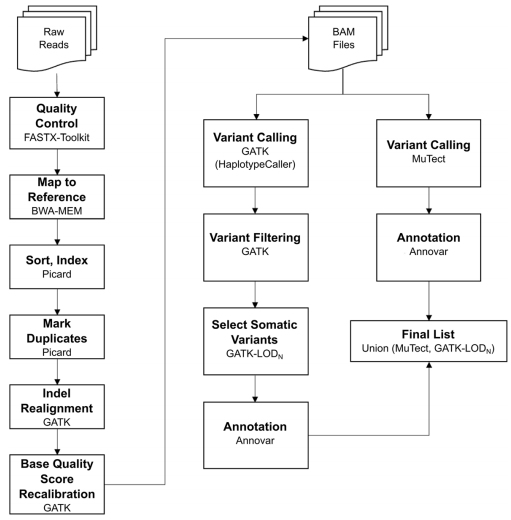
\includegraphics[scale=0.3]{GATK-LODn.png}
\end{figure}
\end{block}
\end{column}
\end{columns}
\end{frame}

\subsection{NGS}
\begin{frame}
\begin{columns}
\begin{column}{0.8\linewidth}
\begin{block}{Next Generation Sequencing}
\begin{itemize}
\item Comprende le nuove tecniche per il sequenziamento del 
DNA.
%\item Succede al Human Genome Project.
\item Tecniche più rapide e meno costose dei metodi precedenti.
\item Shotgun Sequencing.
\end{itemize}
\end{block}
\begin{block}{}
Gli algoritmi di analisi sui dati di NGS sono basati anche sulla teoria dei network.
\end{block}
\end{column}
\end{columns}
\end{frame}

\subsection{Interesse di GATK-LODn}
\begin{frame}
\begin{columns}
\begin{column}{0.8\linewidth}
\begin{block}{Studio sulle varianti}
\begin{itemize}
\item Confronto con il genoma di riferimento.
\item Individuazione delle mutazioni somatiche sia nel tessuto sano del paziente che in quello tumorale.
\item Ricerca di quelle mutazioni che sono presenti solo nel tumore.
\item Confronto tumori simili tra diversi soggetti.
\end{itemize}
\end{block}
\end{column}
\end{columns}
\end{frame}

\section{Materiali e Metodi}

\subsection{Lavoro}
\begin{frame}
\begin{columns}
\begin{column}{0.8\linewidth}
\begin{block}{Lavoro svolto per la tesi}
\begin{itemize}
\item \textbf{Reimplementazione di una parte di GATK-LOD\ped{n} nel tool Snakemake}.
\item Scritti i file di configurazione per il programma.
\item Scritto uno script per l'estrazioni di subset.
\item Scritto uno script per raggruppare i dati.
\item Creato l'installer.
\item Creato uno script che automatizzi l'intero procedimento.
\item Effettuate le simulazioni.
\item Analisi dei dati.
\end{itemize}
\end{block}
\end{column}
\end{columns}
\end{frame}

%\subsection{Struttura delle simulazioni}
%\begin{frame}
%\begin{columns}
%\begin{column}{0.8\linewidth}	
%\begin{block}{Struttura delle simulazioni}
%Una parte di GATK-LOD\ped{n} è stata reimplementata nel tool Snakemake.
%\begin{figure}[H]
%\centering
%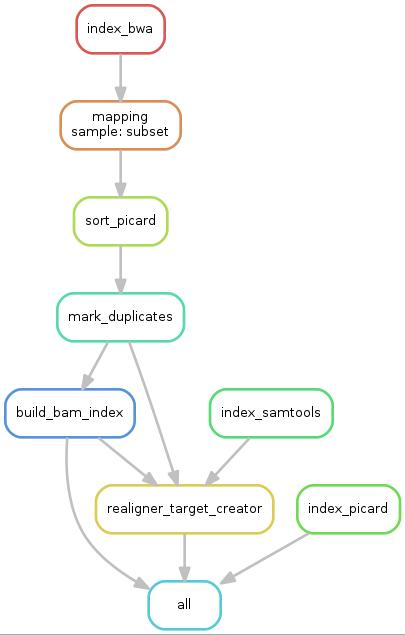
\includegraphics[scale=0.3]{Workflow.jpg}
%\end{figure}
%\end{block}
%\end{column}
%\end{columns}
%\end{frame}

\subsection{La parte considerata}
\begin{frame}
\begin{columns}
\begin{column}{0.8\linewidth}
\begin{block}{Regole indipendenti dal paziente}
Indicizzazione del genoma di riferimento per:
\begin{itemize}
\item BWA
\item Picard
\item Samtools(e GATK) 
\end{itemize}
\end{block}
\begin{block}{Regole dipendenti dal paziente}
\begin{itemize}
\item \textbf{Mapping}: mappatura delle sequenze del paziente sul riferimento.
\item \textbf{Sort Picard}: riordinamento dei file. 
\item \textbf{Mark Duplicates}: identificazione dei duplicati.
\item \textbf{Build BAM}: indicizza i file per velocizzare l'analisi.
\item \textbf{Realigner}: determina gli intervalli che necessitano del riallineamento.
\end{itemize}
\end{block}
\end{column}
\end{columns}
\end{frame}

\subsection{Snakemake}
\begin{frame}
\begin{columns}
\begin{column}{0.8\linewidth}
\begin{block}{Snakemake}
\begin{itemize}
\item Sistema di gestione dei flussi di lavoro
\item Pochi requisiti 
\item Gestione specifica delle risorse
\item Permette di eseguire su cluster
\end{itemize}
\end{block}
\end{column}
\end{columns}
\end{frame}


\subsection{Utilizzo delle risorse}
\begin{frame}
\begin{columns}
\begin{column}{0.8\linewidth}
\begin{block}{Procedura tradizionale}
\begin{figure}[H]
\centering
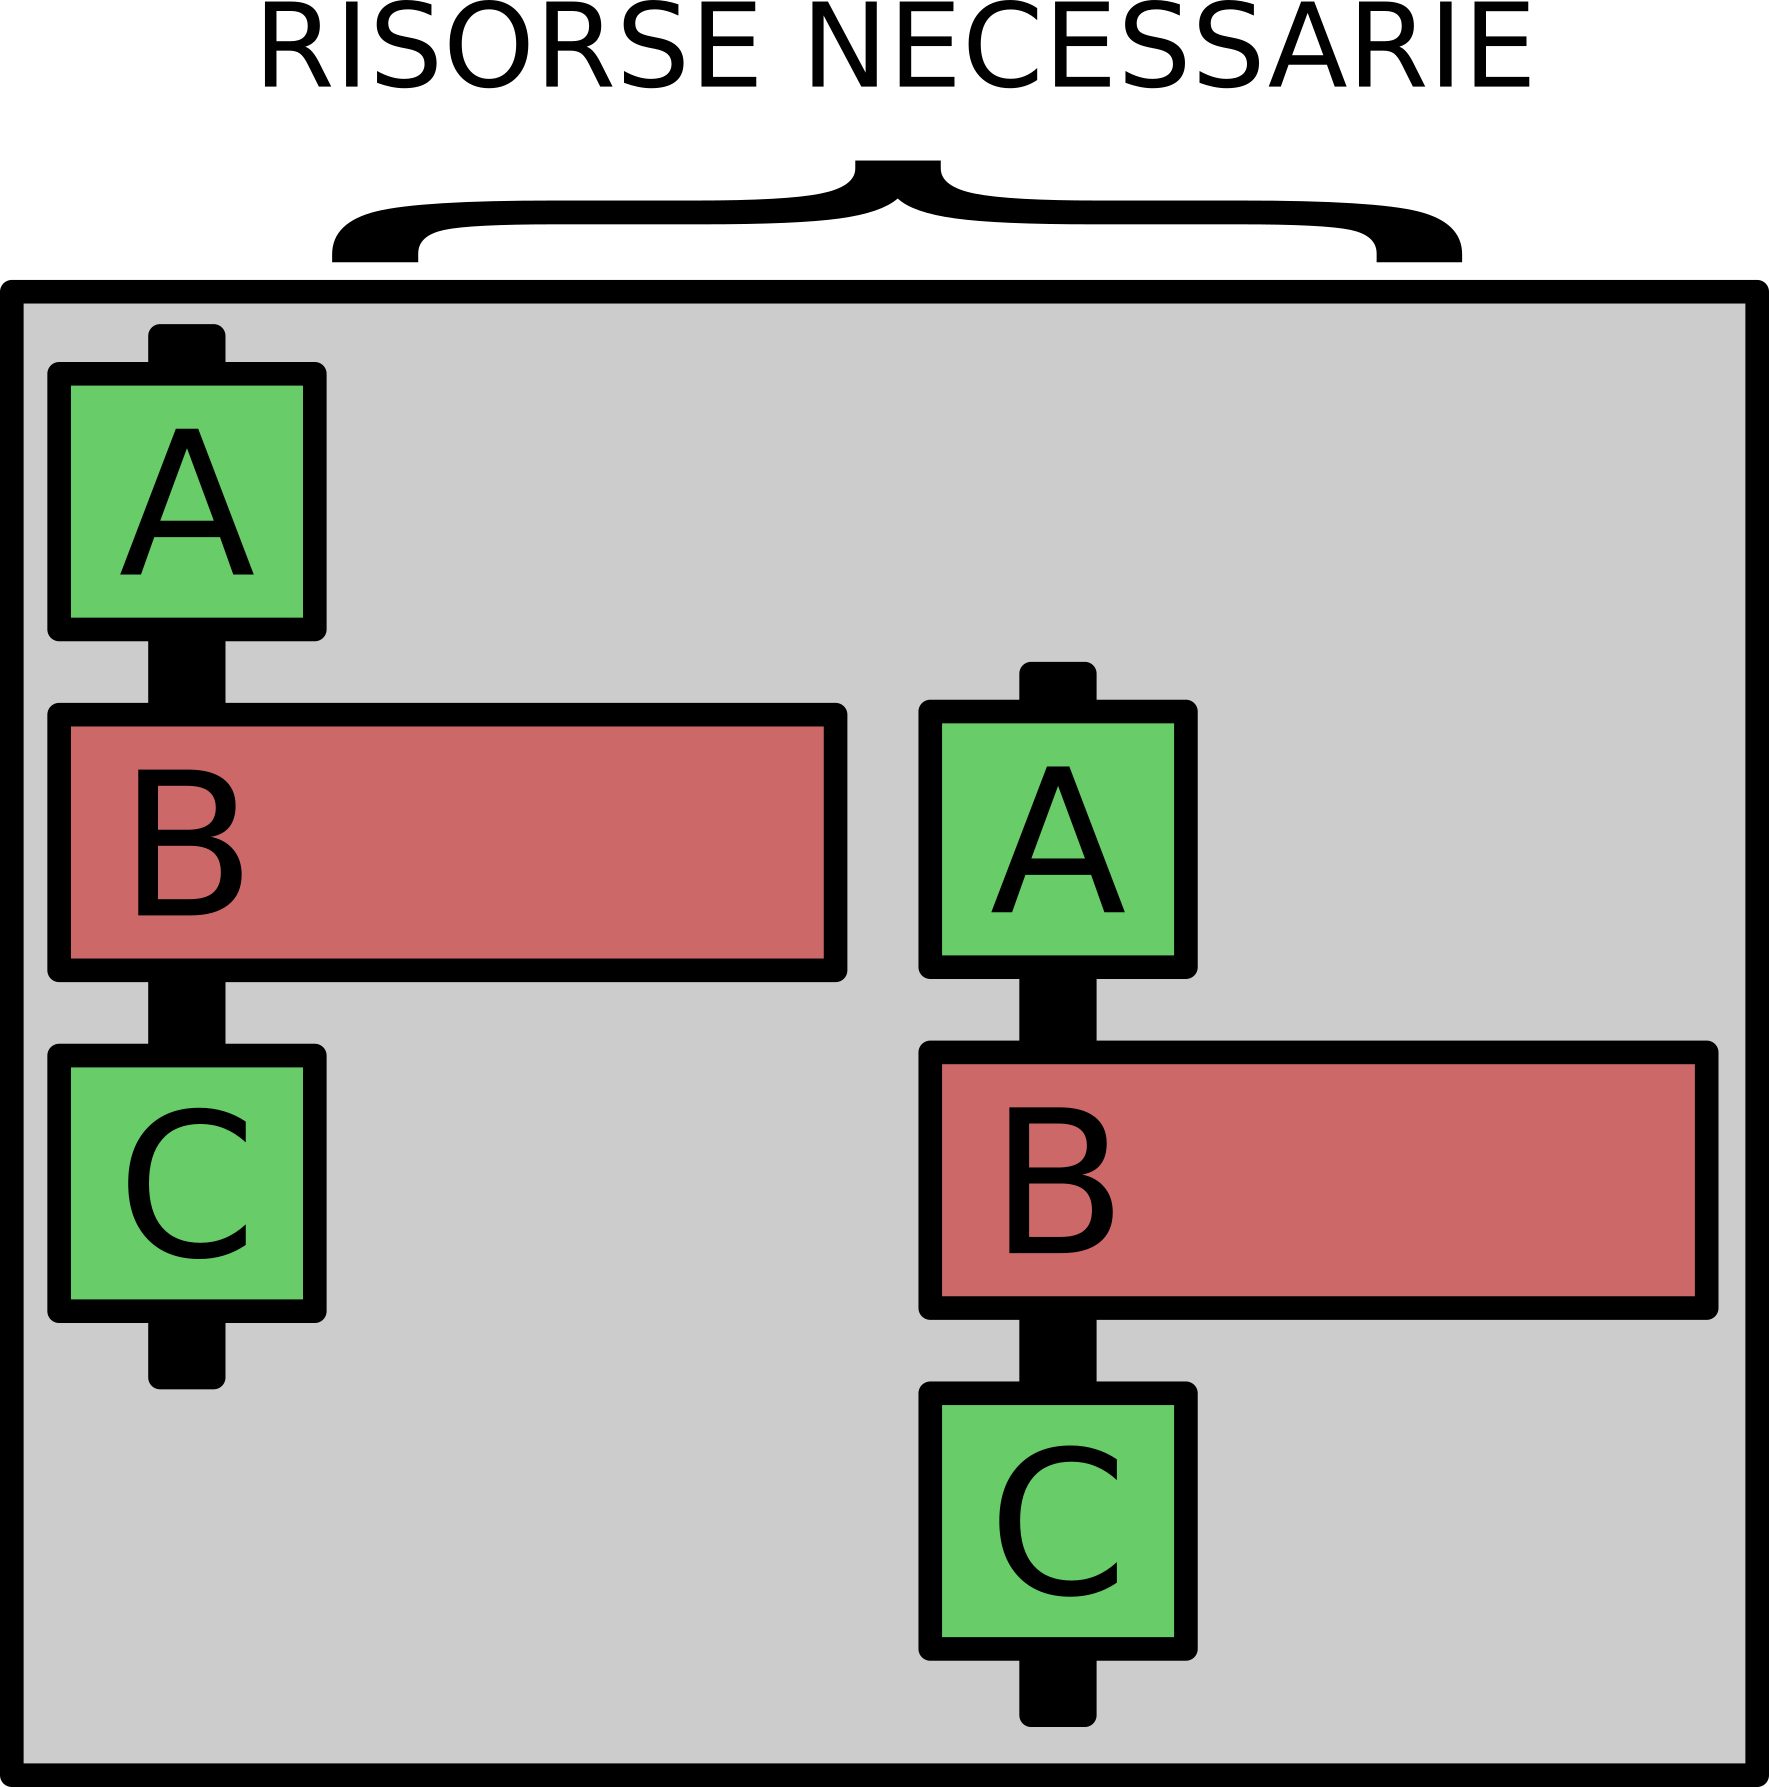
\includegraphics[scale=0.3]{concurrency1.png}
\end{figure}
\end{block}
\end{column}
\end{columns}
\end{frame}

\begin{frame}
\begin{columns}
\begin{column}{0.8\linewidth}
\begin{block}{Procedura ricercata}
\begin{figure}[H]
\centering
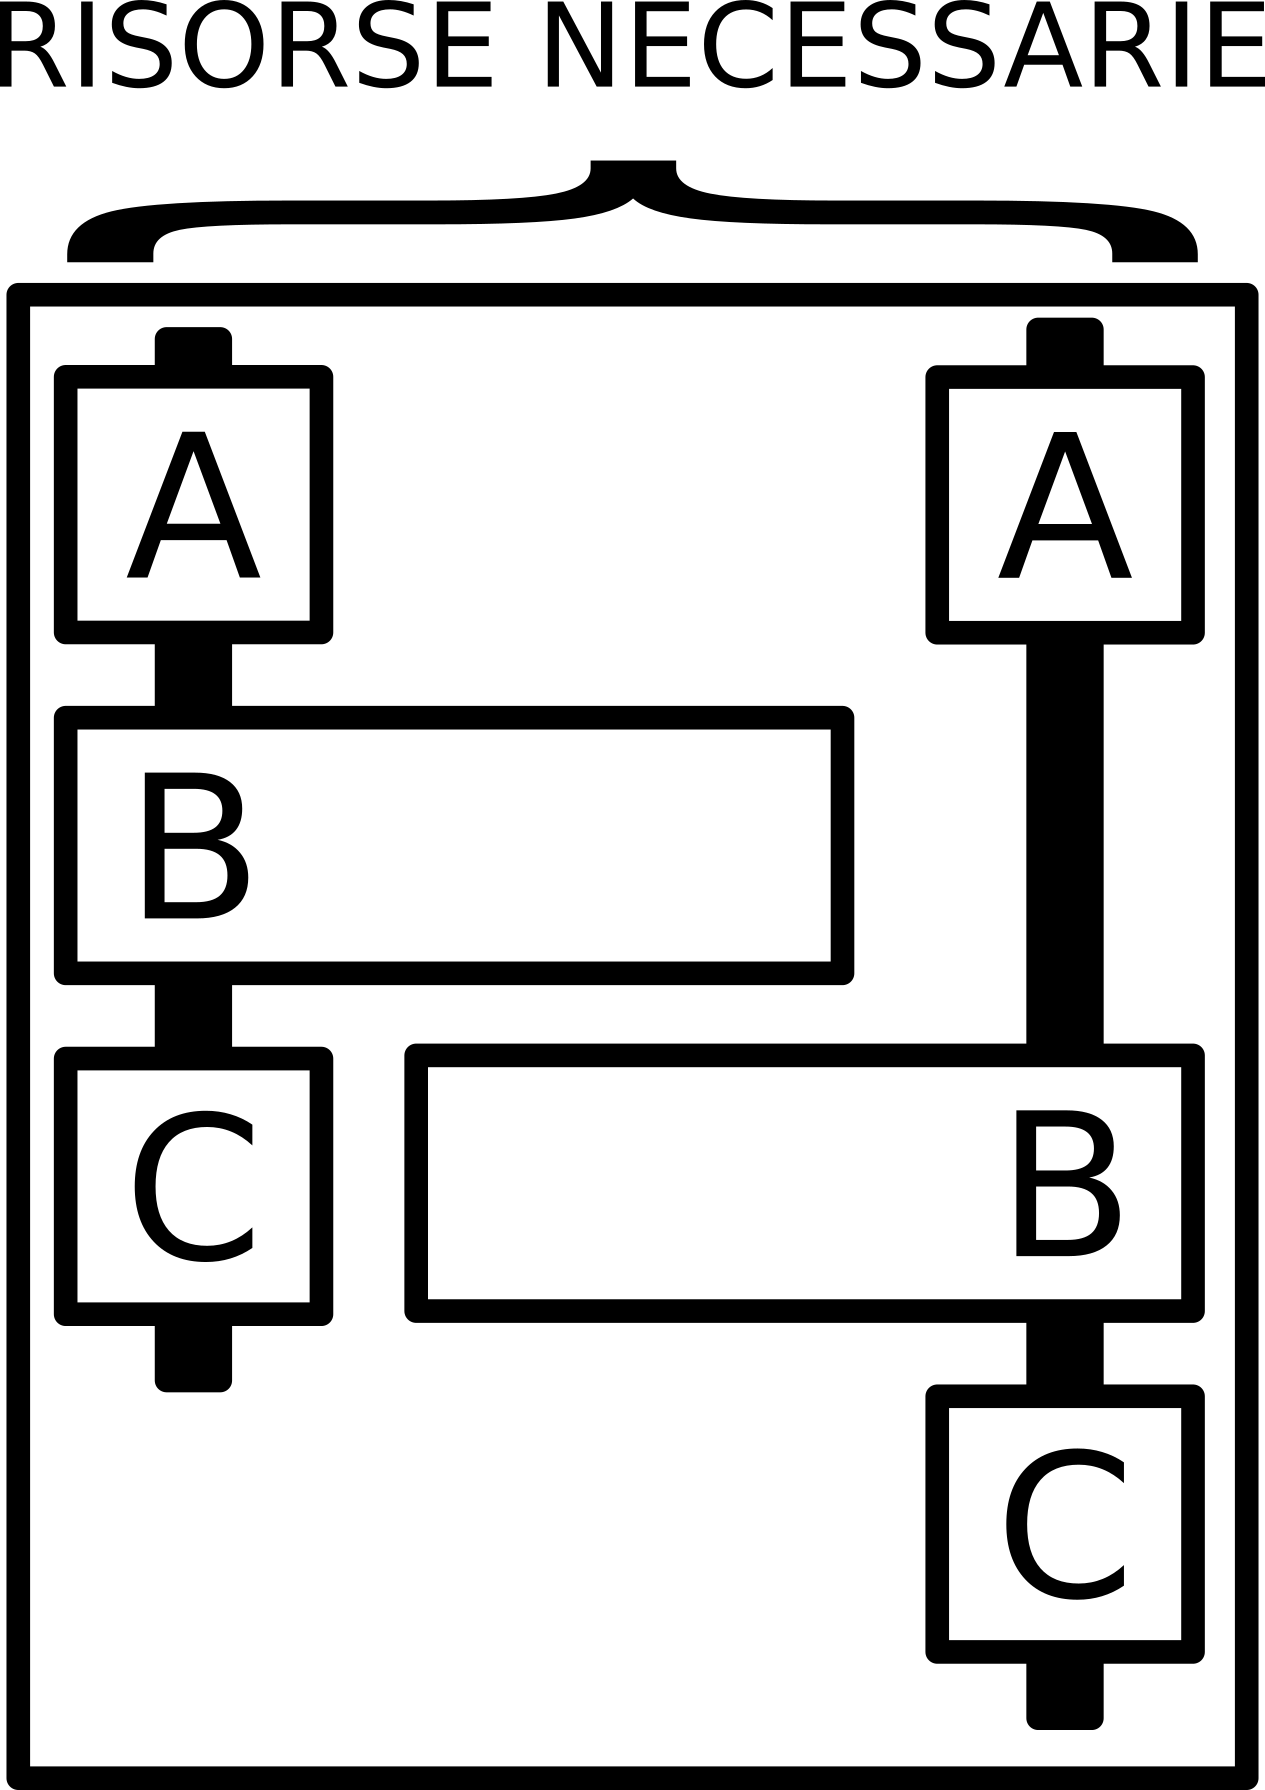
\includegraphics[scale=0.3]{concurrency2.png}
\end{figure}
\end{block}
\end{column}
\end{columns}
\end{frame}



\subsection{Analisi statistiche}
\begin{frame}
\begin{columns}
\begin{column}{0.8\linewidth}	
\begin{block}{Analisi effettuate}
\begin{itemize}
\item Tempo di esecuzione
\item Memoria utilizzata
\end{itemize}
\end{block}
\begin{block}{Simulazioni effettuate}
\begin{table}[H]
	\centering
	\begin{tabular}{lr}
		\toprule
			\text{numero di letture} & \text{dimensione su disco} \\
		\midrule
			\num{1e5}   & \text{2x 28.4\,MB} \\
			\num{1e6}     & \text{2x 284.9\,MB} \\
			\num{3e6}     & \text{2x 854.9\,MB} \\
			\num{9e6}     & \text{2x 2.6\,GB} \\
		\midrule
		\rowcolor{yellow}		
			\num{4.5e7}    & \text{2x 12.8\,GB} \\
		\bottomrule
	\end{tabular}
	\caption{Stima della dimensione dei subset in relazione al numero di letture. L'ultimo valore si riferisce all'intero paziente.}
\end{table}
\end{block}
\end{column}
\end{columns}
\end{frame}

\subsection{I nodi utilizzati}
\begin{frame}
\begin{columns}
\begin{column}{0.8\linewidth}
\begin{table}[H]
\begin{threeparttable}
\resizebox{1.0\textwidth}{!}{%
$\begin{array}{*{6}{c}}
	\toprule
		Nodo & CPU & Memory & Storage & Costo\text{*} & Consumo\text{*}  \\
	\midrule
		xeond & \text{1x Xeon D-1540} & 16\,GB & 8\,TB(HDD) & \text{\euro 1000} & 60\,W\\
		avoton & \text{1x Atom C2750}  & 16\,GB & 5\,TB(HDD) & \text{\euro 600} & 30\,W\\
		n3700 & \text{1x Pentium N3700}  & 8\,GB & 0.5\,TB(SSD) & \text{\euro 130} & 8\,W \\
	\midrule
	\rowcolor{yellow}		
		bio8 & \text{2x Xeon E5-2620v4} & 128\,GB & 2\,TB(HDD) & \text{\euro 10000} & 180\,W\\		
	\bottomrule
\end{array}$%
}
\begin{tablenotes}\footnotesize
\item[*] I valori di costo e consumo energetico sono stimati.
\end{tablenotes}
\end{threeparttable}
\caption{Caratteristiche dei nodi.}
\label{tab:cluster_generali}
\end{table}

\begin{table}[H]
\centering
\resizebox{1.0\textwidth}{!}{%
$\begin{array}{*{6}{c}}
	\toprule
		CPU & Microarchitecture(Platform)/litho & Freq(GHz) & Cores & Cache & TDP\\
	\midrule
		\text{Xeon D-1540} & Broadwell/14nm & 2.0(2.60) & 8(16) & 12\,MB & 45\,W \\
		\text{Atom C2750} & Silvermont(Avoton)/22nm & 2.40(2.60) & 8 & 4\,MB & 25\,W \\
		\text{Pentium N3700} & Airmont(Braswell)/14nm & 1.60(2.40) & 4 & 2\,MB & 6\,W \\
	\midrule
	\rowcolor{yellow}	
		\text{Xeon E5-2620v4} & Broadwell-EP/14nm & 2.10(3.00) & 8(16) & 20\,MB & 85\,W \\
	\bottomrule
\end{array}$%
}
\caption{Caratteristiche delle CPU.}
\label{tab:cpu}
\end{table}
\end{column}
\end{columns}
\end{frame}

\section{Risultati}
\subsection{Tempo di esecuzione}
%\begin{frame}
%\begin{columns}
%\begin{column}{0.8\linewidth}	
%\begin{figure}[H]
%\centering
%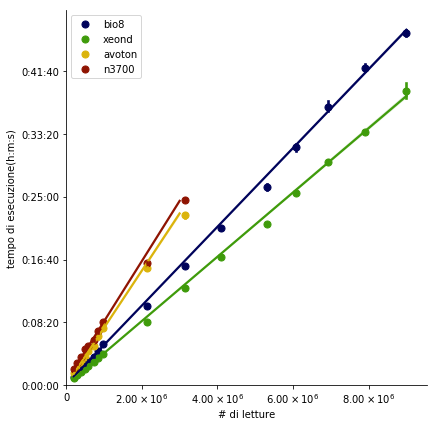
\includegraphics[scale=0.5]{mapping.png}	
%\captionof{figure}{Tempi per Mapping.}
%\label{subfig:Map}
%\end{figure}
%\end{column}
%\end{columns}
%\end{frame}

\begin{frame}
\begin{columns}
\begin{column}{0.8\linewidth}	
\begin{figure}[H]
\centering
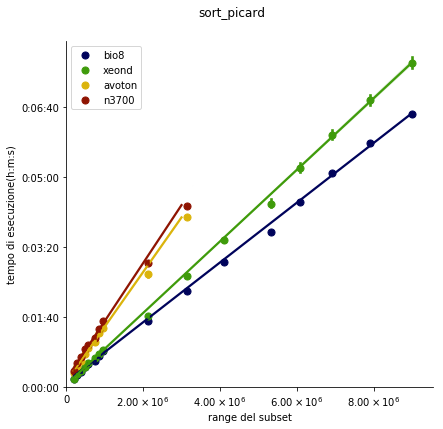
\includegraphics[scale=0.5]{sort_picard.png}
\captionof{figure}{Tempi per Sort Picard.}
\label{subfig:SP}
\end{figure}
\end{column}
\end{columns}
\end{frame}

\begin{frame}
\begin{columns}
\begin{column}{0.8\linewidth}	
\begin{figure}[H]
\centering
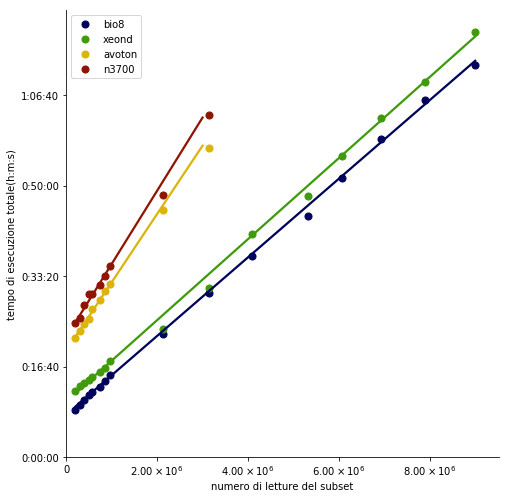
\includegraphics[scale=0.43]{Tempi_complessivi.png}
\captionof{figure}{Tempi complessivi.}
\label{subfig:SP}
\end{figure}
\end{column}
\end{columns}
\end{frame}


\subsection{Memoria utilizzata}
%\begin{frame}
%\begin{columns}
%\begin{column}{0.8\linewidth}	
%\begin{figure}[H]
%\centering
%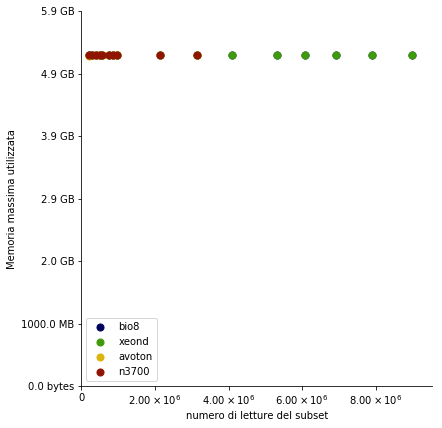
\includegraphics[scale=0.46]{Max_rss_mapping.png}
%\caption{Mapping.}
%\label{fig:RSSind}
%\end{figure}
%\end{column}
%\end{columns}
%\end{frame}

%\begin{frame}
%\begin{columns}
%\begin{column}{0.8\linewidth}	
%\begin{figure}[H]
%\centering
%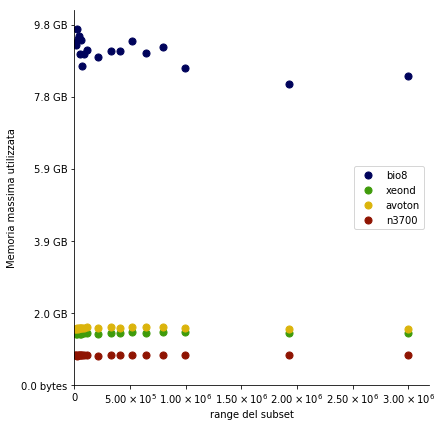
\includegraphics[scale=0.46]{Max_rss_realigner.png}
%\caption{Realigner.}
%\label{fig:RSSind}
%\end{figure}
%\end{column}
%\end{columns}
%\end{frame}


\begin{frame}
\begin{columns}
\begin{column}{0.8\linewidth}	
\begin{figure}[H]
\centering
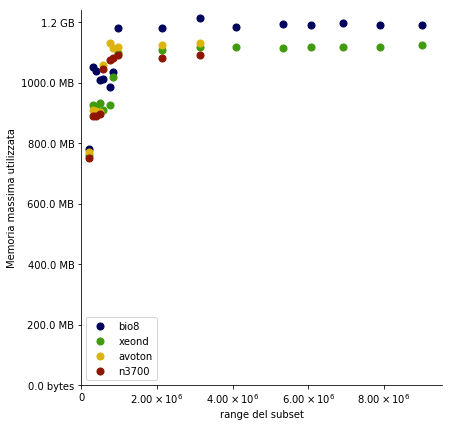
\includegraphics[scale=0.46]{Max_rss_sort_picard.png}
\caption{Sort Picard.}
\label{fig:RSSind}
\end{figure}
\end{column}
\end{columns}
\end{frame}

\section{Conclusioni}
\begin{frame}
\begin{columns}
\begin{column}{0.8\linewidth}	
\begin{block}{Tempo di esecuzione}
\begin{itemize}
\item avoton e n3700 impiegano il doppio del tempo
\item xeond è comparabile a bio8 consumando un terzo dell'energia e costando 10 volte di meno
\end{itemize}
\end{block}
\begin{block}{Memoria utilizzata}
\begin{itemize}
\item Saturazione
\item Valori di saturazioni consistenti
\item Sempre inferiore al massimo di memoria accessibile
\end{itemize}
\end{block}
\end{column}
\end{columns}
\end{frame}

\subsection{Conclusione}
\begin{frame}
\begin{columns}
\begin{column}{0.8\linewidth}	
\begin{block}{Conclusione}
\textbf{In base a questi risultati questa pipeline di calcolo bioinformatico sembra
essere realisticamente eseguibile anche su nodi a bassa potenza senza una
perdita considerevole di prestazioni.}
\end{block}
\end{column}
\end{columns}
\end{frame}

\subsection{Sviluppo futuro}
\begin{frame}
\begin{columns}
\begin{column}{0.8\linewidth}	
\begin{block}{Sviluppo futuro}
\begin{itemize}
\item Simulazioni a core multipli sui singoli nodi
\item Completamento della pipeline
\item Simulazioni su cluster
\end{itemize}
\end{block}
\begin{block}{}
Una volta terminati questi passi intendiamo pubblicarli.
\end{block}
\end{column}
\end{columns}
\end{frame}

\end{document}

